\documentclass[a4paper,12pt]{report}
\usepackage{graphicx}
\usepackage{listings}
\title{Tugas pemrograman 2}
\author{idam fadilah}
\date{23 oktober 2019}
\begin{document}
\maketitle
\chapter{Python}
\section{Variabel}
\paragraph{}
Variabel adalah sebuah tempat untuk menampung value dimemori, ibaratkan sebuah ruangan atau wadah,  variabel dibagi dua berdasarkan ruang lingkup yaitu variable lokal dan global, untuk menentukan variabel global atau lokal itu tergantung dari tempat dideklarasikannya variabel pada program yang sedang dibuat. Variabel global yaitu variabel yang dapat diakses di semua lingkup  dalam program yang sedang dibuat, dalam kata lain variabel global ini dapat dikenali oleh semua fungsi dan prosedur, sementara variabel lokal yaitu variabel yang dapat diakses hanya di lingkup khusus, dalam kata lain variabel lokal ini hanya bisa diakses pada fungsi/prosedur dimana variabel itu dideklarasikan.\\ \\
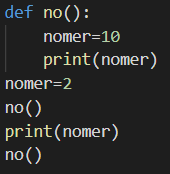
\includegraphics[scale=1]{images/variabel.png} 
\section{Input dan output}
\paragraph{}
\graphicspath{{images}}
Input \& output tentunya wajib kita ketahui agar pengguna dan program dapat berinteraksi, berikut merupakan sintax meminta inputan :\\
\begin{itemize}
	\item var \= input(“message”)\\
\end{itemize}
var yaitu variabel yang akan menampung inputan dari user, input merupakan fungsi yang digunakan untuk menangkap inputan dari user, message digunakan untuk mencetak suatu keterangan saat meminta inputan, contoh :\\
\begin{itemize}
	\item nama = input(“Masukan nama anda : ”)\\
\end{itemize}
sementara untuk menampilkan data bisa menggunakan fungsi print(), contoh :\\
print(“Halo galaksi”)\\
atau kalian juga bisa menampilkan isi suatu variabel, untuk menampilkan data variabel yaitu dengan menuliskan nama variabel tanpa tanda petik, contoh :\\
\begin{itemize}
	\item nama=”Idam fadilah”\\
print(nama)\\
\end{itemize}
atau mungkin digabung  yaitu dengan menambahkan koma untuk memisahkan antara message dengan variabel, contoh :\\
\begin{itemize}
	\item nama=”idam fadilah”\\
print(“Halo ”,nama,” Selamat datang di galaksi bima sakti”)\\
\end{itemize}
\section{Operasi aritmatika dan casting}
\subsection{Operasi aritmatika}
\paragraph{}
Sebagai bahasa pemrograman, pastinya python mempunyai operasi aritmatika antara lain seperti tambah, kurang kali, bagi.  symbol yang digunakan dalam operasi aritmatikanya pun tidak jauh berbeda dengan rekan-rekannya.  berikut merupakan contoh penggunaan operasi aritmatika pada python
Contoh misalkan disini kita mempunyai variable : a=7 dan b=3\\
\subsection{Casting}
\paragraph{}
Namun apa yang akan terjadi bila mana ternyata variabel a merupakan string dan variabel b merupakan integer, contoh a=”7” dan b=3, tentu program akan melemparkan error bukan? Disinilah peran casting digunakan. Casting yaitu cara/mekanisme untuk mengubah tipe data dari suatu data primitive, maksudnya gimana? Jadi misalkan kita akan menjumlahkan variabel a dan b seperti contoh diatas tetapi logikanya sebuah kata (string) tidak akan bisa dijumlahkan dengan angka (“7” + 3) karena variabel a diapit oleh tanda kutip, ini berarti variabel a bertipe data string untuk itu kita perlu merubah dulu variabel a yang tadinya string menjadi integer. Berikut adalah sintax untuk melakukan casting :
\begin{itemize}
	\item int(var/value) : mengubah tipe data ke integer, contoh int(angka)
	\item float(var/value) : mengubah tipe data ke float, contoh float(hasil)
	\item string(var/value) : mengubah tipe data ke str, contoh string(12)
\end{itemize}
jadi cara menyelesaikan contoh kasus diatas yaitu dengan menggunakan int() untuk merubah tipe data variabel a menjadi integer, contoh :
\begin{itemize}

\item a=”7”\\
b=3\\
int(a)+b\\

\end{itemize}
maka jika dijalankan program diatas tidak akan error, karena tipe data dari variabel a sudah diubah dari string menjadi integer sehingga program dapat dijalankan dengan lancar

\section{condision (kondisi)}
\paragraph{}
Pengambilan keputusan kadang diperlukan dalam sebuah program untuk menentukan tindakan apa yang akan dilakukan sesuai dengan kondisi yang terjadi, contoh kasus misalkan ada seorang anak bernama idam, seorang manusia biasa yang membutuhkan makan, jika idam lapar maka idam akan makan. Maka dapat dipecah seperti dibawah ini :\\

Kondisi, jika :\\
Idam lapar\\
Maka :\\
Idam akan makan\\

Namun kadang kondisi tidak juga sampai disitu, kadang ada saja tambahan opsi sebuah kondisi, misalkan jika idam makan maka idam hidup, namun jika tidak maka idam akan mati. Maka dapat dipecah seperti ini :\\

Kondisi, jika :\\
Idam makan\\
Maka :\\
Idam akan hidup\\
Jika tidak :\\
Idam akan mati\\
	
Contoh diatas dapat ditulis dalam sintax python dengan menggunakan if, pengkondisiian if dalam python dibagi menjadi 4, yaitu : if, if else, elif, nested if. Berikut merupakan pembahasannya :
\subsection{if}
\paragraph{}
if digunakan jika misalkan kita mempunyai kondisi yang sederhana.\\ \\
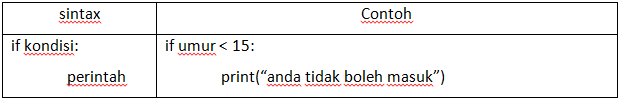
\includegraphics[scale=1]{images/if.png} 
\subsection{if else}
\paragraph{}
If else digunakan jika kita mempunyai kondisi namun jika kondisi tidak terpenuhi maka kita akan melakukan sesuatu yang lain, penggunaan else dalam kondisi tidak diwajibkan, digunakan hanya jika diperlukan.\\ \\
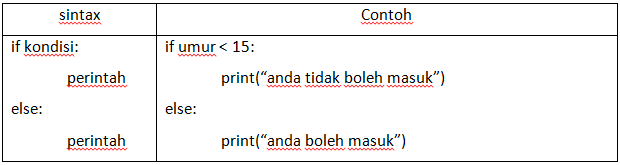
\includegraphics[scale=1]{images/if else.png} 
\subsection{elif}
\paragraph{}
Elif digunakan jika kita mempunyai 2 atau lebih opsi kondisi\\ \\
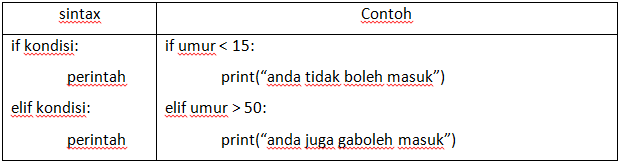
\includegraphics[scale=1]{images/elif.png} 
\subsection{nested if}
\paragraph{}
Nested if/if berserang atau disebut juga if dalam if, digunakan jika misal kita mempunyai
Kondisi yang ingin ditambahkan jika kondisi sebelumnya sudah terpenuhi\\ \\
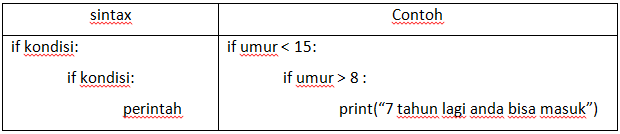
\includegraphics[scale=1]{images/nested if.png} 
\section{loop (perulangan)}
\paragraph{}
Dalam membuat sebuah program, kadang kita perlu satu baris atau satu blok kode beberapa kali, misalkan kita membuat program input nama jika misal namanya salah maka program akan meminta inputan lagi, bagaimana jika misalkan user salah input nama  10 kali atau mungkin lebih tentu kita harus menyiapkan banyak sekali kode. disini fungsi perulangan dipakai, perulangan dalam python ada 2 yaitu for dan while.
\subsection{for}
\paragraph{}
perulangan yang sudah diketahui akhirnya, pada perulangan ini wajib mencantumkan batas perulangan\\
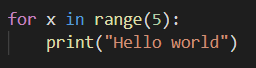
\includegraphics[scale=1]{images/for.png} 
\subsection{while}
\paragraph{}
perulangan yang akan terus mengulang selama kondisi true\\
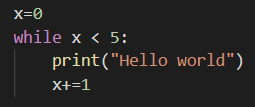
\includegraphics[scale=1]{images/while.png} 
\section{Error}
\paragraph{}
Error yang didapat :
\begin{itemize}
	\item IndexError: string index out of range\\
	penanganan errornya bisa menggunakan while dan fungsi len() untuk memastikan panjang NPM yang di inputkan memiliki panjang yang sama dengan yang ditetapkan
	\item TypeError: unsupported operand type(s) for +: 'int' and 'str'\\
	penanganan error ini bisa ditangani menggunakan casting operand kedua menjadi integer
	\item TypeError: can only concatenate str (not "int") to str\\
	penanganan error ini bisa ditangani menggunakan casting operand kedua menjadi string
\end{itemize}
\section{Try Except}
\paragraph{}
 dalam membuat sebuah program pasti ada saja kode yang membuat program crash saat dijalan kan, contoh jika kita menuliskan 2/0 dalam program maka program akan error, salah satu cara menangani nya yaitu dengan menggunakan statement try except, contoh penggunaan :\\ \\
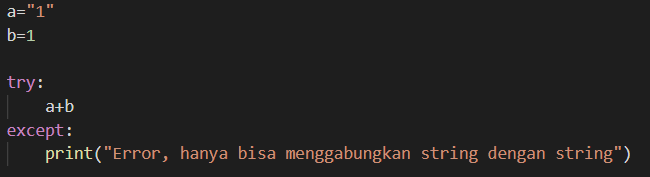
\includegraphics[scale=1]{images/try except.png} 
\chapter{Latihan soal}
\section{Soal}
\subsection{Soal 1}
\lstinputlisting[language=Python]{src/NPM1.py}
\subsection{Soal 2}
\lstinputlisting[language=Python]{src/NPM2.py}
\subsection{Soal 3}
\lstinputlisting[language=Python]{src/NPM3.py}
\subsection{Soal 4}
\lstinputlisting[language=Python]{src/NPM4.py}
\subsection{Soal 5}
\lstinputlisting[language=Python]{src/NPM5.py}
\subsection{Soal 6}
\lstinputlisting[language=Python]{src/NPM6.py}
\subsection{Soal 7}
\lstinputlisting[language=Python]{src/NPM7.py}
\subsection{Soal 8}
\lstinputlisting[language=Python]{src/NPM8.py}
\subsection{Soal 9}
\lstinputlisting[language=Python]{src/NPM9.py}
\subsection{Soal 10}
\lstinputlisting[language=Python]{src/NPM10.py}
\subsection{Soal 11}
\lstinputlisting[language=Python]{src/NPM11.py}
\subsection{Soal 2err}
\lstinputlisting[language=Python]{src/2err.py}









\end{document}